\documentclass[12pt,a4paper]{article}
\usepackage[utf8]{inputenc}
\usepackage[T2A]{fontenc}
\usepackage[russian]{babel}
\usepackage{amsmath,amssymb}
\usepackage{geometry}
\geometry{left=2cm,right=2cm,top=2cm,bottom=2cm}
\usepackage{enumitem}
\usepackage{hyperref}
\usepackage{graphicx}



\begin{document}

\begin{titlepage}
\centering

{\large Министерство образования и науки Российской Федерации\par}

\vspace{1cm}

{\large\textbf{Саратовский государственный технический университет}\par}
{\large\textbf{имени Гагарина Ю.А.}\par}

\vspace{2cm}

{\large Практическая работа\par}

\vspace{0.3cm}

{\large по курсу «Методы обработки сигналов и изображений»\par}

\vspace{0.3cm}

{\large для студентов направления\par}
{\large «Информационные системы и технологии»\par}

\vspace{2cm}

{\large\textbf{Базовые параметры изображений}\par}
\vspace{0.2cm}
{\large\textbf{Морфологические преобразования}\par}
\vspace{0.2cm}
{\large\textbf{Фильтрация изображений. Работа с контурами}\par}
\vspace{0.2cm}
{\large\textbf{Яркостные преобразования}\par}
\vspace{0.2cm}
{\large\textbf{Сопоставление изображений. Работа с видео}\par}

\vfill

\begin{flushright}
\begin{minipage}{0.45\textwidth}
\raggedright
Выполнил:\par
студент м1-ИФСТ-21\par
Тащилин Антон Александрович\par

\vspace{0.5cm}

Проверил:\par
ст. преподаватель\par
Пиминов Дмитрий Алексеевич\par
\end{minipage}
\end{flushright}

\vfill

{\large Саратов 2026\par}

\end{titlepage}

\section{Глубина цвета: определение и анализ}

\textbf{Глубина цвета} (битовая глубина, разрядность, \textit{color depth}) --- это параметр цифрового изображения, определяющий количество бит, используемых для кодирования цвета или тона каждого отдельного пикселя. Этот показатель влияет на количество уникальных цветов или оттенков серого, которые могут быть представлены в изображении, и на плавность цветовых переходов и точность воспроизведения тонального диапазона.

Математическая зависимость между глубиной цвета \(I\) (в битах) и количеством возможных цветов \(K\) выражается формулой:
\[
K = 2^I
\]

Примеры:
\begin{itemize}
    \item \textbf{1 бит:} \(2^1 = 2\) цвета. Используется для штриховой графики (чёрно-белой).
    \item \textbf{8 бит:} \(2^8 = 256\) цветов. Применяется для изображений в градациях серого или индексированных палитр (например, формат GIF).
    \item \textbf{24 бита (True Color):} 8 бит на каждый из трёх цветовых каналов (красный, зелёный, синий). \(2^{24} = 16\,777\,216\) цветов. Это стандарт для большинства цифровых фотографий и мониторов.
    \item \textbf{32 бита:} часто это 24 бита цвета плюс 8-битный альфа-канал, отвечающий за прозрачность пикселя.
    \item \textbf{48 бит и выше:} 16 бит на канал. Используется в профессиональной фотографии (RAW-формат) и полиграфии. Такая глубина позволяет сохранить больше информации в светах и тенях, что необходимо для последующей обработки, цветокоррекции и предотвращения эффекта постеризации (ступенчатых переходов на градиентах).
\end{itemize}

\section{Формулы перевода между цветовыми моделями (30 формул)}

\textbf{Предварительные условия.}

Исходные значения R, G, B в модели RGB имеют диапазон \(0..255\). Перед всеми вычислениями они нормализуются делением на 255:
\[
R' = \frac{R}{255},\quad G' = \frac{G}{255},\quad B' = \frac{B}{255},
\]
и далее в формулах используются именно нормализованные значения \(R', G', B' \in [0, 1]\). Если результат обратного перехода даёт \(R', G', B' \in [0, 1]\), то для получения значений в диапазоне \(0..255\) их умножают на 255: \(R = 255 R'\), \(G = 255 G'\), \(B = 255 B'\).

Для CMYK значения C, M, Y, K --- в диапазоне \([0, 1]\).
Для LAB значения L --- в \([0, 100]\), a и b --- примерно в \([-128, 127]\).
Для всех формул используется стандартное цветовое пространство sRGB с гамма-коррекцией \(\gamma = 2.2\) (упрощённо) и точкой белого D65.

\subsection{Блок 1. Из модели RGB}

\textbf{1. RGB \(\to\) CMYK.}

Значения R, G, B делятся на 255, чтобы перейти от диапазона \(0..255\) к диапазону \(0..1\):
\[
R' = \frac{R}{255},\quad G' = \frac{G}{255},\quad B' = \frac{B}{255}
\]
Цвет чёрного ключа (K) рассчитывается из красного (\(R'\)), зелёного (\(G'\)) и синего (\(B'\)) цветов:
\[
K = 1 - \max(R', G', B')
\]
Голубой цвет (C) рассчитывается из красного (\(R'\)) и чёрного (\(K\)) цветов:
\[
C = \frac{1 - R' - K}{1 - K}
\]
Пурпурный цвет (M) рассчитывается из зелёного (\(G'\)) и чёрного (\(K\)) цветов:
\[
M = \frac{1 - G' - K}{1 - K}
\]
Жёлтый цвет (Y) рассчитывается из синего (\(B'\)) и чёрного (\(K\)) цветов:
\[
Y = \frac{1 - B' - K}{1 - K}
\]
Если \(K = 1\), то \(C = M = Y = 0\).

\textbf{2. RGB \(\to\) HSL.}

Нормализация:
\[
R' = \frac{R}{255},\quad G' = \frac{G}{255},\quad B' = \frac{B}{255}
\]
Светлота (L) вычисляется как полусумма максимума и минимума из \(R', G', B'\):
\[
L = \frac{\max(R', G', B') + \min(R', G', B')}{2}
\]
Насыщенность (S):
\[
S = \begin{cases}
0, & \text{если } \max(R', G', B') = \min(R', G', B') \\[8pt]
\dfrac{\max(R', G', B') - \min(R', G', B')}{1 - |2L - 1|}, & \text{иначе}
\end{cases}
\]
Тон (H):
\[
H = \begin{cases}
0, & \text{если } \max(R', G', B') = \min(R', G', B') \\[8pt]
60^\circ \cdot \left( \dfrac{G' - B'}{\max(R', G', B') - \min(R', G', B')} \bmod 6 \right), & \text{если } \max(R', G', B') = R' \\[12pt]
60^\circ \cdot \left( \dfrac{B' - R'}{\max(R', G', B') - \min(R', G', B')} + 2 \right), & \text{если } \max(R', G', B') = G' \\[12pt]
60^\circ \cdot \left( \dfrac{R' - G'}{\max(R', G', B') - \min(R', G', B')} + 4 \right), & \text{если } \max(R', G', B') = B'
\end{cases}
\]

\textbf{3. RGB \(\to\) HSV.}

Нормализация:
\[
R' = \frac{R}{255},\quad G' = \frac{G}{255},\quad B' = \frac{B}{255}
\]
Яркость (V):
\[
V = \max(R', G', B')
\]
Насыщенность (S):
\[
S = \begin{cases}
0, & \text{если } \max(R', G', B') = 0 \\[8pt]
\dfrac{\max(R', G', B') - \min(R', G', B')}{\max(R', G', B')}, & \text{иначе}
\end{cases}
\]
Тон (H) вычисляется по тем же правилам, что и в HSL:
\[
H = \begin{cases}
0, & \text{если } \max(R', G', B') = \min(R', G', B') \\[8pt]
60^\circ \cdot \left( \dfrac{G' - B'}{\max(R', G', B') - \min(R', G', B')} \bmod 6 \right), & \text{если } \max(R', G', B') = R' \\[12pt]
60^\circ \cdot \left( \dfrac{B' - R'}{\max(R', G', B') - \min(R', G', B')} + 2 \right), & \text{если } \max(R', G', B') = G' \\[12pt]
60^\circ \cdot \left( \dfrac{R' - G'}{\max(R', G', B') - \min(R', G', B')} + 4 \right), & \text{если } \max(R', G', B') = B'
\end{cases}
\]

\textbf{4. RGB \(\to\) LAB (через XYZ).}

Нормализация:
\[
R' = \frac{R}{255},\quad G' = \frac{G}{255},\quad B' = \frac{B}{255}
\]
Линеаризация каждого канала:
\[
R_{lin} = \begin{cases} \dfrac{R'}{12.92}, & R' \le 0.04045 \\[8pt] \left( \dfrac{R' + 0.055}{1.055} \right)^{2.4}, & \text{иначе} \end{cases}
\]
\[
G_{lin} = \begin{cases} \dfrac{G'}{12.92}, & G' \le 0.04045 \\[8pt] \left( \dfrac{G' + 0.055}{1.055} \right)^{2.4}, & \text{иначе} \end{cases}
\]
\[
B_{lin} = \begin{cases} \dfrac{B'}{12.92}, & B' \le 0.04045 \\[8pt] \left( \dfrac{B' + 0.055}{1.055} \right)^{2.4}, & \text{иначе} \end{cases}
\]
Переход в XYZ (матрица sRGB):
\begin{align*}
X &= 0.4124 \cdot R_{lin} + 0.3576 \cdot G_{lin} + 0.1805 \cdot B_{lin} \\
Y &= 0.2126 \cdot R_{lin} + 0.7152 \cdot G_{lin} + 0.0722 \cdot B_{lin} \\
Z &= 0.0193 \cdot R_{lin} + 0.1192 \cdot G_{lin} + 0.9505 \cdot B_{lin}
\end{align*}
Нормализация относительно точки белого D65:
\[
X_n = 95.047,\quad Y_n = 100.0,\quad Z_n = 108.883
\]
\[
x = \frac{X}{X_n},\quad y = \frac{Y}{Y_n},\quad z = \frac{Z}{Z_n}
\]
Функция нелинейности:
\[
f(t) = \begin{cases}
t^{1/3}, & t > \left(\dfrac{6}{29}\right)^3 \\[8pt]
\dfrac{1}{3} \cdot \left(\dfrac{29}{6}\right)^2 \cdot t + \dfrac{4}{29}, & \text{иначе}
\end{cases}
\]
Итоговые компоненты:
\begin{align*}
L &= 116 \cdot f(y) - 16 \\
a &= 500 \cdot (f(x) - f(y)) \\
b &= 200 \cdot (f(y) - f(z))
\end{align*}

\textbf{5. RGB \(\to\) YCbCr (ITU-R BT.601, полный диапазон).}

Нормализация:
\[
R' = \frac{R}{255},\quad G' = \frac{G}{255},\quad B' = \frac{B}{255}
\]
\begin{align*}
Y &= 0.299 \cdot R' + 0.587 \cdot G' + 0.114 \cdot B' \\
Cb &= 0.564 \cdot (B' - Y) + 0.5 \\
Cr &= 0.713 \cdot (R' - Y) + 0.5
\end{align*}

\textbf{6. RGB \(\to\) YCbCr (ITU-R BT.601, студийный диапазон 16--235).}

Нормализация:
\[
R' = \frac{R}{255},\quad G' = \frac{G}{255},\quad B' = \frac{B}{255}
\]
\begin{align*}
Y &= 0.257 \cdot R' + 0.504 \cdot G' + 0.098 \cdot B' + 0.0625 \\
Cb &= -0.148 \cdot R' - 0.291 \cdot G' + 0.439 \cdot B' + 0.5 \\
Cr &= 0.439 \cdot R' - 0.368 \cdot G' - 0.071 \cdot B' + 0.5
\end{align*}

\subsection{Блок 2. Из модели CMYK}

\textbf{7. CMYK \(\to\) RGB.}

\begin{align*}
R' &= (1 - C) \cdot (1 - K) \\
G' &= (1 - M) \cdot (1 - K) \\
B' &= (1 - Y) \cdot (1 - K)
\end{align*}
Для получения значений в диапазоне \(0..255\): \(R = 255 \cdot R'\), \(G = 255 \cdot  G'\), \(B = 255 \cdot B'\).

\textbf{8. CMYK \(\to\) HSL (через RGB).}

Шаг 1. CMYK \(\to\) RGB:
\begin{align*}
R' &= (1 - C) \cdot (1 - K) \\
G' &= (1 - M) \cdot (1 - K) \\
B' &= (1 - Y) \cdot (1 - K)
\end{align*}
Шаг 2. RGB \(\to\) HSL:
\[
L = \frac{\max(R', G', B') + \min(R', G', B')}{2}
\]
\[
S = \begin{cases}
0, & \text{если } \max(R', G', B') = \min(R', G', B') \\[8pt]
\dfrac{\max(R', G', B') - \min(R', G', B')}{1 - |2L - 1|}, & \text{иначе}
\end{cases}
\]
\[
H = \begin{cases}
0, & \text{если } \max(R', G', B') = \min(R', G', B') \\[8pt]
60^\circ \cdot \left( \dfrac{G' - B'}{\max(R', G', B') - \min(R', G', B')} \bmod 6 \right), & \text{если } \max(R', G', B') = R' \\[12pt]
60^\circ \cdot \left( \dfrac{B' - R'}{\max(R', G', B') - \min(R', G', B')} + 2 \right), & \text{если } \max(R', G', B') = G' \\[12pt]
60^\circ \cdot \left( \dfrac{R' - G'}{\max(R', G', B') - \min(R', G', B')} + 4 \right), & \text{если } \max(R', G', B') = B'
\end{cases}
\]

\textbf{9. CMYK \(\to\) HSV (через RGB).}

Шаг 1. CMYK \(\to\) RGB:
\begin{align*}
R' &= (1 - C) \cdot (1 - K) \\
G' &= (1 - M) \cdot (1 - K) \\
B' &= (1 - Y) \cdot (1 - K)
\end{align*}
Шаг 2. RGB \(\to\) HSV:
\[
V = \max(R', G', B')
\]
\[
S = \begin{cases}
0, & \text{если } \max(R', G', B') = 0 \\[8pt]
\dfrac{\max(R', G', B') - \min(R', G', B')}{\max(R', G', B')}, & \text{иначе}
\end{cases}
\]
\[
H = \begin{cases}
0, & \text{если } \max(R', G', B') = \min(R', G', B') \\[8pt]
60^\circ \cdot \left( \dfrac{G' - B'}{\max(R', G', B') - \min(R', G', B')} \bmod 6 \right), & \text{если } \max(R', G', B') = R' \\[12pt]
60^\circ \cdot \left( \dfrac{B' - R'}{\max(R', G', B') - \min(R', G', B')} + 2 \right), & \text{если } \max(R', G', B') = G' \\[12pt]
60^\circ \cdot \left( \dfrac{R' - G'}{\max(R', G', B') - \min(R', G', B')} + 4 \right), & \text{если } \max(R', G', B') = B'
\end{cases}
\]

\textbf{10. CMYK \(\to\) LAB (через RGB).}

Шаг 1. CMYK \(\to\) RGB:
\begin{align*}
R' &= (1 - C) \cdot (1 - K) \\
G' &= (1 - M) \cdot (1 - K) \\
B' &= (1 - Y) \cdot (1 - K)
\end{align*}
Шаг 2. RGB \(\to\) LAB (линеаризация и переход в XYZ):
\[
R_{lin} = \begin{cases} \dfrac{R'}{12.92}, & R' \le 0.04045 \\[8pt] \left( \dfrac{R' + 0.055}{1.055} \right)^{2.4}, & \text{иначе} \end{cases}
\]
\[
G_{lin} = \begin{cases} \dfrac{G'}{12.92}, & G' \le 0.04045 \\[8pt] \left( \dfrac{G' + 0.055}{1.055} \right)^{2.4}, & \text{иначе} \end{cases}
\]
\[
B_{lin} = \begin{cases} \dfrac{B'}{12.92}, & B' \le 0.04045 \\[8pt] \left( \dfrac{B' + 0.055}{1.055} \right)^{2.4}, & \text{иначе} \end{cases}
\]
\begin{align*}
X &= 0.4124 \cdot R_{lin} + 0.3576 \cdot G_{lin} + 0.1805 \cdot B_{lin} \\
Y &= 0.2126 \cdot R_{lin} + 0.7152 \cdot G_{lin} + 0.0722 \cdot B_{lin} \\
Z &= 0.0193 \cdot R_{lin} + 0.1192 \cdot G_{lin} + 0.9505 \cdot B_{lin}
\end{align*}
\[
x = \frac{X}{X_n},\quad y = \frac{Y}{Y_n},\quad z = \frac{Z}{Z_n},\quad X_n = 95.047,\ Y_n = 100.0,\ Z_n = 108.883
\]
\[
f(t) = \begin{cases} t^{1/3}, & t > \left(\dfrac{6}{29}\right)^3 \\[8pt] \dfrac{1}{3} \cdot \left(\dfrac{29}{6}\right)^2 \cdot t + \dfrac{4}{29}, & \text{иначе} \end{cases}
\]
\begin{align*}
L &= 116 \cdot f(y) - 16 \\
a &= 500 \cdot (f(x) - f(y)) \\
b &= 200 \cdot (f(y) - f(z))
\end{align*}

\textbf{11. CMYK \(\to\) YCbCr (через RGB).}

Шаг 1. CMYK \(\to\) RGB:
\begin{align*}
R' &= (1 - C) \cdot (1 - K) \\
G' &= (1 - M) \cdot (1 - K) \\
B' &= (1 - Y) \cdot (1 - K)
\end{align*}
Шаг 2. RGB \(\to\) YCbCr (BT.601, полный диапазон):
\begin{align*}
Y &= 0.299 \cdot R' + 0.587 \cdot G' + 0.114 \cdot B' \\
Cb &= 0.564 \cdot (B' - Y) + 0.5 \\
Cr &= 0.713 \cdot (R' - Y) + 0.5
\end{align*}

\subsection{Блок 3. Из модели HSL}

\textbf{12. HSL \(\to\) RGB.}

\[
C = (1 - |2L - 1|) \cdot S,\quad H' = \frac{H}{60},\quad X = C \cdot (1 - |H' \bmod 2 - 1|),\quad m = L - \frac{C}{2}
\]
Компоненты \(R', G', B'\) выбираются по диапазону \(H'\):
\begin{align*}
&0 \le H' < 1: & R' &= C + m,\quad G' = X + m,\quad B' = m \\
&1 \le H' < 2: & R' &= X + m,\quad G' = C + m,\quad B' = m \\
&2 \le H' < 3: & R' &= m,\quad G' = C + m,\quad B' = X + m \\
&3 \le H' < 4: & R' &= m,\quad G' = X + m,\quad B' = C + m \\
&4 \le H' < 5: & R' &= X + m,\quad G' = m,\quad B' = C + m \\
&5 \le H' < 6: & R' &= C + m,\quad G' = m,\quad B' = X + m
\end{align*}
Для получения значений \(0..255\): \(R = 255 R'\), \(G = 255 G'\), \(B = 255 B'\).

\textbf{13. HSL \(\to\) CMYK (через RGB).}

Шаг 1. HSL \(\to\) RGB:
\[
C = (1 - |2L - 1|) \cdot S,\quad H' = \frac{H}{60},\quad X = C \cdot (1 - |H' \bmod 2 - 1|),\quad m = L - \frac{C}{2}
\]
\begin{align*}
&0 \le H' < 1: & R' &= C + m,\quad G' = X + m,\quad B' = m \\
&1 \le H' < 2: & R' &= X + m,\quad G' = C + m,\quad B' = m \\
&2 \le H' < 3: & R' &= m,\quad G' = C + m,\quad B' = X + m \\
&3 \le H' < 4: & R' &= m,\quad G' = X + m,\quad B' = C + m \\
&4 \le H' < 5: & R' &= X + m,\quad G' = m,\quad B' = C + m \\
&5 \le H' < 6: & R' &= C + m,\quad G' = m,\quad B' = X + m
\end{align*}
Шаг 2. RGB \(\to\) CMYK:
\begin{align*}
K &= 1 - \max(R', G', B') \\
C &= \frac{1 - R' - K}{1 - K},\quad M = \frac{1 - G' - K}{1 - K},\quad Y = \frac{1 - B' - K}{1 - K}
\end{align*}
Если \(K = 1\), то \(C = M = Y = 0\).

\textbf{14. HSL \(\to\) HSV.}

\begin{align*}
V &= L + S \cdot \min(L, 1 - L) \\
S_v &= \begin{cases} 0, & \text{если } V = 0 \\[8pt] 2 \cdot \left( 1 - \dfrac{L}{V} \right), & \text{иначе} \end{cases} \\
H_v &= H
\end{align*}

\textbf{15. HSL \(\to\) LAB (через RGB).}

Шаг 1. HSL \(\to\) RGB:
\[
C = (1 - |2L - 1|) \cdot S,\quad H' = \frac{H}{60},\quad X = C \cdot (1 - |H' \bmod 2 - 1|),\quad m = L - \frac{C}{2}
\]
\begin{align*}
&0 \le H' < 1: & R' &= C + m,\quad G' = X + m,\quad B' = m \\
&1 \le H' < 2: & R' &= X + m,\quad G' = C + m,\quad B' = m \\
&2 \le H' < 3: & R' &= m,\quad G' = C + m,\quad B' = X + m \\
&3 \le H' < 4: & R' &= m,\quad G' = X + m,\quad B' = C + m \\
&4 \le H' < 5: & R' &= X + m,\quad G' = m,\quad B' = C + m \\
&5 \le H' < 6: & R' &= C + m,\quad G' = m,\quad B' = X + m
\end{align*}
Шаг 2. RGB \(\to\) LAB:
\[
R_{lin} = \begin{cases} \dfrac{R'}{12.92}, & R' \le 0.04045 \\[8pt] \left( \dfrac{R' + 0.055}{1.055} \right)^{2.4}, & \text{иначе} \end{cases}
\]
\[
G_{lin} = \begin{cases} \dfrac{G'}{12.92}, & G' \le 0.04045 \\[8pt] \left( \dfrac{G' + 0.055}{1.055} \right)^{2.4}, & \text{иначе} \end{cases}
\]
\[
B_{lin} = \begin{cases} \dfrac{B'}{12.92}, & B' \le 0.04045 \\[8pt] \left( \dfrac{B' + 0.055}{1.055} \right)^{2.4}, & \text{иначе} \end{cases}
\]
\begin{align*}
X &= 0.4124 \cdot R_{lin} + 0.3576 \cdot G_{lin} + 0.1805 \cdot B_{lin} \\
Y &= 0.2126 \cdot R_{lin} + 0.7152 \cdot G_{lin} + 0.0722 \cdot B_{lin} \\
Z &= 0.0193 \cdot R_{lin} + 0.1192 \cdot G_{lin} + 0.9505 \cdot B_{lin}
\end{align*}
\[
x = \frac{X}{X_n},\quad y = \frac{Y}{Y_n},\quad z = \frac{Z}{Z_n},\quad X_n = 95.047,\ Y_n = 100.0,\ Z_n = 108.883
\]
\[
f(t) = \begin{cases} t^{1/3}, & t > \left(\dfrac{6}{29}\right)^3 \\[8pt] \dfrac{1}{3} \cdot \left(\dfrac{29}{6}\right)^2 \cdot t + \dfrac{4}{29}, & \text{иначе} \end{cases}
\]
\begin{align*}
L &= 116 \cdot f(y) - 16 \\
a &= 500 \cdot (f(x) - f(y)) \\
b &= 200 \cdot (f(y) - f(z))
\end{align*}

\textbf{16. HSL \(\to\) YCbCr (через RGB).}

Шаг 1. HSL \(\to\) RGB:
\[
C = (1 - |2L - 1|) \cdot S,\quad H' = \frac{H}{60},\quad X = C \cdot (1 - |H' \bmod 2 - 1|),\quad m = L - \frac{C}{2}
\]
\begin{align*}
&0 \le H' < 1: & R' &= C + m,\quad G' = X + m,\quad B' = m \\
&1 \le H' < 2: & R' &= X + m,\quad G' = C + m,\quad B' = m \\
&2 \le H' < 3: & R' &= m,\quad G' = C + m,\quad B' = X + m \\
&3 \le H' < 4: & R' &= m,\quad G' = X + m,\quad B' = C + m \\
&4 \le H' < 5: & R' &= X + m,\quad G' = m,\quad B' = C + m \\
&5 \le H' < 6: & R' &= C + m,\quad G' = m,\quad B' = X + m
\end{align*}
Шаг 2. RGB \(\to\) YCbCr (BT.601, полный диапазон):
\begin{align*}
Y &= 0.299 \cdot R' + 0.587 \cdot G' + 0.114 \cdot B' \\
Cb &= 0.564 \cdot (B' - Y) + 0.5 \\
Cr &= 0.713 \cdot (R' - Y) + 0.5
\end{align*}

\subsection{Блок 4. Из модели HSV}

\textbf{17. HSV \(\to\) RGB.}

\[
C = V \cdot S,\quad H' = \frac{H}{60},\quad X = C \cdot (1 - |H' \bmod 2 - 1|),\quad m = V - C
\]
\begin{align*}
&0 \le H' < 1: & R' &= C + m,\quad G' = X + m,\quad B' = m \\
&1 \le H' < 2: & R' &= X + m,\quad G' = C + m,\quad B' = m \\
&2 \le H' < 3: & R' &= m,\quad G' = C + m,\quad B' = X + m \\
&3 \le H' < 4: & R' &= m,\quad G' = X + m,\quad B' = C + m \\
&4 \le H' < 5: & R' &= X + m,\quad G' = m,\quad B' = C + m \\
&5 \le H' < 6: & R' &= C + m,\quad G' = m,\quad B' = X + m
\end{align*}
Для получения значений \(0..255\): \(R = 255 R'\), \(G = 255 G'\), \(B = 255 B'\).

\textbf{18. HSV \(\to\) CMYK (через RGB).}

Шаг 1. HSV \(\to\) RGB:
\[
C = V \cdot S,\quad H' = \frac{H}{60},\quad X = C \cdot (1 - |H' \bmod 2 - 1|),\quad m = V - C
\]
\begin{align*}
&0 \le H' < 1: & R' &= C + m,\quad G' = X + m,\quad B' = m \\
&1 \le H' < 2: & R' &= X + m,\quad G' = C + m,\quad B' = m \\
&2 \le H' < 3: & R' &= m,\quad G' = C + m,\quad B' = X + m \\
&3 \le H' < 4: & R' &= m,\quad G' = X + m,\quad B' = C + m \\
&4 \le H' < 5: & R' &= X + m,\quad G' = m,\quad B' = C + m \\
&5 \le H' < 6: & R' &= C + m,\quad G' = m,\quad B' = X + m
\end{align*}
Шаг 2. RGB \(\to\) CMYK:
\begin{align*}
K &= 1 - \max(R', G', B') \\
C &= \frac{1 - R' - K}{1 - K},\quad M = \frac{1 - G' - K}{1 - K},\quad Y = \frac{1 - B' - K}{1 - K}
\end{align*}
Если \(K = 1\), то \(C = M = Y = 0\).

\textbf{19. HSV \(\to\) HSL.}

\begin{align*}
L &= V \cdot \left( 1 - \frac{S}{2} \right) \\
S_l &= \begin{cases} 0, & \text{если } L = 0 \text{ или } L = 1 \\[8pt] \dfrac{V - L}{\min(L, 1 - L)}, & \text{иначе} \end{cases} \\
H_l &= H
\end{align*}

\textbf{20. HSV \(\to\) LAB (через RGB).}

Шаг 1. HSV \(\to\) RGB:
\[
C = V \cdot S,\quad H' = \frac{H}{60},\quad X = C \cdot (1 - |H' \bmod 2 - 1|),\quad m = V - C
\]
\begin{align*}
&0 \le H' < 1: & R' &= C + m,\quad G' = X + m,\quad B' = m \\
&1 \le H' < 2: & R' &= X + m,\quad G' = C + m,\quad B' = m \\
&2 \le H' < 3: & R' &= m,\quad G' = C + m,\quad B' = X + m \\
&3 \le H' < 4: & R' &= m,\quad G' = X + m,\quad B' = C + m \\
&4 \le H' < 5: & R' &= X + m,\quad G' = m,\quad B' = C + m \\
&5 \le H' < 6: & R' &= C + m,\quad G' = m,\quad B' = X + m
\end{align*}
Шаг 2. RGB \(\to\) LAB:
\[
R_{lin} = \begin{cases} \dfrac{R'}{12.92}, & R' \le 0.04045 \\[8pt] \left( \dfrac{R' + 0.055}{1.055} \right)^{2.4}, & \text{иначе} \end{cases}
\]
\[
G_{lin} = \begin{cases} \dfrac{G'}{12.92}, & G' \le 0.04045 \\[8pt] \left( \dfrac{G' + 0.055}{1.055} \right)^{2.4}, & \text{иначе} \end{cases}
\]
\[
B_{lin} = \begin{cases} \dfrac{B'}{12.92}, & B' \le 0.04045 \\[8pt] \left( \dfrac{B' + 0.055}{1.055} \right)^{2.4}, & \text{иначе} \end{cases}
\]
\begin{align*}
X &= 0.4124 \cdot R_{lin} + 0.3576 \cdot G_{lin} + 0.1805 \cdot B_{lin} \\
Y &= 0.2126 \cdot R_{lin} + 0.7152 \cdot G_{lin} + 0.0722 \cdot B_{lin} \\
Z &= 0.0193 \cdot R_{lin} + 0.1192 \cdot G_{lin} + 0.9505 \cdot B_{lin}
\end{align*}
\[
x = \frac{X}{X_n},\quad y = \frac{Y}{Y_n},\quad z = \frac{Z}{Z_n},\quad X_n = 95.047,\ Y_n = 100.0,\ Z_n = 108.883
\]
\[
f(t) = \begin{cases} t^{1/3}, & t > \left(\dfrac{6}{29}\right)^3 \\[8pt] \dfrac{1}{3} \cdot \left(\dfrac{29}{6}\right)^2 \cdot t + \dfrac{4}{29}, & \text{иначе} \end{cases}
\]
\begin{align*}
L &= 116 \cdot f(y) - 16 \\
a &= 500 \cdot (f(x) - f(y)) \\
b &= 200 \cdot (f(y) - f(z))
\end{align*}

\textbf{21. HSV \(\to\) YCbCr (через RGB).}

Шаг 1. HSV \(\to\) RGB:
\[
C = V \cdot S,\quad H' = \frac{H}{60},\quad X = C \cdot (1 - |H' \bmod 2 - 1|),\quad m = V - C
\]
\begin{align*}
&0 \le H' < 1: & R' &= C + m,\quad G' = X + m,\quad B' = m \\
&1 \le H' < 2: & R' &= X + m,\quad G' = C + m,\quad B' = m \\
&2 \le H' < 3: & R' &= m,\quad G' = C + m,\quad B' = X + m \\
&3 \le H' < 4: & R' &= m,\quad G' = X + m,\quad B' = C + m \\
&4 \le H' < 5: & R' &= X + m,\quad G' = m,\quad B' = C + m \\
&5 \le H' < 6: & R' &= C + m,\quad G' = m,\quad B' = X + m
\end{align*}
Шаг 2. RGB \(\to\) YCbCr (BT.601, полный диапазон):
\begin{align*}
Y &= 0.299 \cdot R' + 0.587 \cdot G' + 0.114 \cdot B' \\
Cb &= 0.564 \cdot (B' - Y) + 0.5 \\
Cr &= 0.713 \cdot (R' - Y) + 0.5
\end{align*}

\subsection{Блок 5. Из модели LAB}

\textbf{22. LAB \(\to\) RGB (через XYZ).}

\[
y = \frac{L + 16}{116},\quad x = \frac{a}{500} + y,\quad z = y - \frac{b}{200}
\]
\[
f^{-1}(t) = \begin{cases} t^3, & t > \dfrac{6}{29} \\[8pt] 3 \cdot \left( \dfrac{6}{29} \right)^2 \cdot \left( t - \dfrac{4}{29} \right), & \text{иначе} \end{cases}
\]
\[
X = X_n \cdot f^{-1}(x),\quad Y = Y_n \cdot f^{-1}(y),\quad Z = Z_n \cdot f^{-1}(z)
\]
\[
X_n = 95.047,\quad Y_n = 100.0,\quad Z_n = 108.883
\]
Обратная матрица sRGB:
\begin{align*}
C_R &= 3.2406 \cdot X - 1.5372 \cdot Y - 0.4986 \cdot Z \\
C_G &= -0.9689 \cdot X + 1.8758 \cdot Y + 0.0415 \cdot Z \\
C_B &= 0.0557 \cdot X - 0.2040 \cdot Y + 1.0570 \cdot Z
\end{align*}
Гамма-коррекция:
\[
R' = \begin{cases} 12.92 \cdot C_R, & C_R \le 0.0031308 \\[8pt] 1.055 \cdot C_R^{1/2.4} - 0.055, & \text{иначе} \end{cases}
\]
\[
G' = \begin{cases} 12.92 \cdot C_G, & C_G \le 0.0031308 \\[8pt] 1.055 \cdot C_G^{1/2.4} - 0.055, & \text{иначе} \end{cases}
\]
\[
B' = \begin{cases} 12.92 \cdot C_B, & C_B \le 0.0031308 \\[8pt] 1.055 \cdot C_B^{1/2.4} - 0.055, & \text{иначе} \end{cases}
\]
Для получения значений \(0..255\): \(R = 255 R'\), \(G = 255 G'\), \(B = 255 B'\).

\textbf{23. LAB \(\to\) CMYK (через RGB).}

Шаг 1. LAB \(\to\) RGB (см. полное описание в пункте 22):
\[
y = \frac{L + 16}{116},\quad x = \frac{a}{500} + y,\quad z = y - \frac{b}{200}
\]
\[
f^{-1}(t) = \begin{cases} t^3, & t > \dfrac{6}{29} \\[8pt] 3 \cdot \left( \dfrac{6}{29} \right)^2 \cdot \left( t - \dfrac{4}{29} \right), & \text{иначе} \end{cases}
\]
\[
X = X_n \cdot f^{-1}(x),\quad Y = Y_n \cdot f^{-1}(y),\quad Z = Z_n \cdot f^{-1}(z)
\]
\[
X_n = 95.047,\quad Y_n = 100.0,\quad Z_n = 108.883
\]
\begin{align*}
C_R &= 3.2406 \cdot X - 1.5372 \cdot Y - 0.4986 \cdot Z \\
C_G &= -0.9689 \cdot X + 1.8758 \cdot Y + 0.0415 \cdot Z \\
C_B &= 0.0557 \cdot X - 0.2040 \cdot Y + 1.0570 \cdot Z
\end{align*}
\[
R' = \begin{cases} 12.92 \cdot C_R, & C_R \le 0.0031308 \\[8pt] 1.055 \cdot C_R^{1/2.4} - 0.055, & \text{иначе} \end{cases}
\]
\[
G' = \begin{cases} 12.92 \cdot C_G, & C_G \le 0.0031308 \\[8pt] 1.055 \cdot C_G^{1/2.4} - 0.055, & \text{иначе} \end{cases}
\]
\[
B' = \begin{cases} 12.92 \cdot C_B, & C_B \le 0.0031308 \\[8pt] 1.055 \cdot C_B^{1/2.4} - 0.055, & \text{иначе} \end{cases}
\]
Шаг 2. RGB \(\to\) CMYK:
\begin{align*}
K &= 1 - \max(R', G', B') \\
C &= \frac{1 - R' - K}{1 - K},\quad M = \frac{1 - G' - K}{1 - K},\quad Y = \frac{1 - B' - K}{1 - K}
\end{align*}
Если \(K = 1\), то \(C = M = Y = 0\).

\textbf{24. LAB \(\to\) HSL (через RGB).}

Шаг 1. LAB \(\to\) RGB:
\[
y = \frac{L + 16}{116},\quad x = \frac{a}{500} + y,\quad z = y - \frac{b}{200}
\]
\[
f^{-1}(t) = \begin{cases} t^3, & t > \dfrac{6}{29} \\[8pt] 3 \cdot \left( \dfrac{6}{29} \right)^2 \cdot \left( t - \dfrac{4}{29} \right), & \text{иначе} \end{cases}
\]
\[
X = X_n \cdot f^{-1}(x),\quad Y = Y_n \cdot f^{-1}(y),\quad Z = Z_n \cdot f^{-1}(z)
\]
\[
X_n = 95.047,\quad Y_n = 100.0,\quad Z_n = 108.883
\]
\begin{align*}
C_R &= 3.2406 \cdot X - 1.5372 \cdot Y - 0.4986 \cdot Z \\
C_G &= -0.9689 \cdot X + 1.8758 \cdot Y + 0.0415 \cdot Z \\
C_B &= 0.0557 \cdot X - 0.2040 \cdot Y + 1.0570 \cdot Z
\end{align*}
\[
R' = \begin{cases} 12.92 \cdot C_R, & C_R \le 0.0031308 \\[8pt] 1.055 \cdot C_R^{1/2.4} - 0.055, & \text{иначе} \end{cases}
\]
\[
G' = \begin{cases} 12.92 \cdot C_G, & C_G \le 0.0031308 \\[8pt] 1.055 \cdot C_G^{1/2.4} - 0.055, & \text{иначе} \end{cases}
\]
\[
B' = \begin{cases} 12.92 \cdot C_B, & C_B \le 0.0031308 \\[8pt] 1.055 \cdot C_B^{1/2.4} - 0.055, & \text{иначе} \end{cases}
\]
Шаг 2. RGB \(\to\) HSL:
\[
L = \frac{\max(R', G', B') + \min(R', G', B')}{2}
\]
\[
S = \begin{cases}
0, & \text{если } \max(R', G', B') = \min(R', G', B') \\[8pt]
\dfrac{\max(R', G', B') - \min(R', G', B')}{1 - |2L - 1|}, & \text{иначе}
\end{cases}
\]
\[
H = \begin{cases}
0, & \text{если } \max(R', G', B') = \min(R', G', B') \\[8pt]
60^\circ \cdot \left( \dfrac{G' - B'}{\max(R', G', B') - \min(R', G', B')} \bmod 6 \right), & \text{если } \max(R', G', B') = R' \\[12pt]
60^\circ \cdot \left( \dfrac{B' - R'}{\max(R', G', B') - \min(R', G', B')} + 2 \right), & \text{если } \max(R', G', B') = G' \\[12pt]
60^\circ \cdot \left( \dfrac{R' - G'}{\max(R', G', B') - \min(R', G', B')} + 4 \right), & \text{если } \max(R', G', B') = B'
\end{cases}
\]

\textbf{25. LAB \(\to\) HSV (через RGB).}

Шаг 1. LAB \(\to\) RGB:
\[
y = \frac{L + 16}{116},\quad x = \frac{a}{500} + y,\quad z = y - \frac{b}{200}
\]
\[
f^{-1}(t) = \begin{cases} t^3, & t > \dfrac{6}{29} \\[8pt] 3 \cdot \left( \dfrac{6}{29} \right)^2 \cdot \left( t - \dfrac{4}{29} \right), & \text{иначе} \end{cases}
\]
\[
X = X_n \cdot f^{-1}(x),\quad Y = Y_n \cdot f^{-1}(y),\quad Z = Z_n \cdot f^{-1}(z)
\]
\[
X_n = 95.047,\quad Y_n = 100.0,\quad Z_n = 108.883
\]
\begin{align*}
C_R &= 3.2406 \cdot X - 1.5372 \cdot Y - 0.4986 \cdot Z \\
C_G &= -0.9689 \cdot X + 1.8758 \cdot Y + 0.0415 \cdot Z \\
C_B &= 0.0557 \cdot X - 0.2040 \cdot Y + 1.0570 \cdot Z
\end{align*}
\[
R' = \begin{cases} 12.92 \cdot C_R, & C_R \le 0.0031308 \\[8pt] 1.055 \cdot C_R^{1/2.4} - 0.055, & \text{иначе} \end{cases}
\]
\[
G' = \begin{cases} 12.92 \cdot C_G, & C_G \le 0.0031308 \\[8pt] 1.055 \cdot C_G^{1/2.4} - 0.055, & \text{иначе} \end{cases}
\]
\[
B' = \begin{cases} 12.92 \cdot C_B, & C_B \le 0.0031308 \\[8pt] 1.055 \cdot C_B^{1/2.4} - 0.055, & \text{иначе} \end{cases}
\]
Шаг 2. RGB \(\to\) HSV:
\[
V = \max(R', G', B')
\]
\[
S = \begin{cases}
0, & \text{если } \max(R', G', B') = 0 \\[8pt]
\dfrac{\max(R', G', B') - \min(R', G', B')}{\max(R', G', B')}, & \text{иначе}
\end{cases}
\]
\[
H = \begin{cases}
0, & \text{если } \max(R', G', B') = \min(R', G', B') \\[8pt]
60^\circ \cdot \left( \dfrac{G' - B'}{\max(R', G', B') - \min(R', G', B')} \bmod 6 \right), & \text{если } \max(R', G', B') = R' \\[12pt]
60^\circ \cdot \left( \dfrac{B' - R'}{\max(R', G', B') - \min(R', G', B')} + 2 \right), & \text{если } \max(R', G', B') = G' \\[12pt]
60^\circ \cdot \left( \dfrac{R' - G'}{\max(R', G', B') - \min(R', G', B')} + 4 \right), & \text{если } \max(R', G', B') = B'
\end{cases}
\]

\textbf{26. LAB \(\to\) YCbCr (через RGB).}

Шаг 1. LAB \(\to\) RGB:
\[
y = \frac{L + 16}{116},\quad x = \frac{a}{500} + y,\quad z = y - \frac{b}{200}
\]
\[
f^{-1}(t) = \begin{cases} t^3, & t > \dfrac{6}{29} \\[8pt] 3 \cdot \left( \dfrac{6}{29} \right)^2 \cdot \left( t - \dfrac{4}{29} \right), & \text{иначе} \end{cases}
\]
\[
X = X_n \cdot f^{-1}(x),\quad Y = Y_n \cdot f^{-1}(y),\quad Z = Z_n \cdot f^{-1}(z)
\]
\[
X_n = 95.047,\quad Y_n = 100.0,\quad Z_n = 108.883
\]
\begin{align*}
C_R &= 3.2406 \cdot X - 1.5372 \cdot Y - 0.4986 \cdot Z \\
C_G &= -0.9689 \cdot X + 1.8758 \cdot Y + 0.0415 \cdot Z \\
C_B &= 0.0557 \cdot X - 0.2040 \cdot Y + 1.0570 \cdot Z
\end{align*}
\[
R' = \begin{cases} 12.92 \cdot C_R, & C_R \le 0.0031308 \\[8pt] 1.055 \cdot C_R^{1/2.4} - 0.055, & \text{иначе} \end{cases}
\]
\[
G' = \begin{cases} 12.92 \cdot C_G, & C_G \le 0.0031308 \\[8pt] 1.055 \cdot C_G^{1/2.4} - 0.055, & \text{иначе} \end{cases}
\]
\[
B' = \begin{cases} 12.92 \cdot C_B, & C_B \le 0.0031308 \\[8pt] 1.055 \cdot C_B^{1/2.4} - 0.055, & \text{иначе} \end{cases}
\]
Шаг 2. RGB \(\to\) YCbCr (BT.601, полный диапазон):
\begin{align*}
Y &= 0.299 \cdot R' + 0.587 \cdot G' + 0.114 \cdot B' \\
Cb &= 0.564 \cdot (B' - Y) + 0.5 \\
Cr &= 0.713 \cdot (R' - Y) + 0.5
\end{align*}

\subsection{Блок 6. Из модели YCbCr}

\textbf{27. YCbCr \(\to\) RGB (ITU-R BT.601, полный диапазон).}

\begin{align*}
R' &= Y + 1.402 \cdot (Cr - 0.5) \\
G' &= Y - 0.344136 \cdot (Cb - 0.5) - 0.714136 \cdot (Cr - 0.5) \\
B' &= Y + 1.772 \cdot (Cb - 0.5)
\end{align*}
Для получения значений \(0..255\): \(R = 255 R'\), \(G = 255 G'\), \(B = 255 B'\).

\textbf{28. YCbCr \(\to\) RGB (ITU-R BT.601, студийный диапазон).}

Шаг 1. Денормализация (приведение к шкале \(0..255\)):
\[
Y_{255} = 219 \cdot Y_{st} + 16,\quad Cb_{255} = 224 \cdot Cb_{st} + 16,\quad Cr_{255} = 224 \cdot Cr_{st} + 16
\]
Шаг 2. Нормализация к диапазону \(0..1\):
\[
Y = \frac{Y_{255}}{255},\quad Cb = \frac{Cb_{255}}{255},\quad Cr = \frac{Cr_{255}}{255}
\]
Шаг 3. Переход в RGB:
\begin{align*}
R' &= Y + 1.402 \cdot (Cr - 0.5) \\
G' &= Y - 0.344136 \cdot (Cb - 0.5) - 0.714136 \cdot (Cr - 0.5) \\
B' &= Y + 1.772 \cdot (Cb - 0.5)
\end{align*}
Для получения значений \(0..255\): \(R = 255 R'\), \(G = 255 G'\), \(B = 255 B'\).

\textbf{29. YCbCr \(\to\) CMYK (через RGB).}

Шаг 1. YCbCr \(\to\) RGB (BT.601, полный диапазон):
\begin{align*}
R' &= Y + 1.402 \cdot (Cr - 0.5) \\
G' &= Y - 0.344136 \cdot (Cb - 0.5) - 0.714136 \cdot (Cr - 0.5) \\
B' &= Y + 1.772 \cdot (Cb - 0.5)
\end{align*}
Шаг 2. RGB \(\to\) CMYK:
\begin{align*}
K &= 1 - \max(R', G', B') \\
C &= \frac{1 - R' - K}{1 - K},\quad M = \frac{1 - G' - K}{1 - K},\quad Y = \frac{1 - B' - K}{1 - K}
\end{align*}
Если \(K = 1\), то \(C = M = Y = 0\).

\textbf{30. YCbCr \(\to\) HSL (через RGB).}

Шаг 1. YCbCr \(\to\) RGB (BT.601, полный диапазон):
\begin{align*}
R' &= Y + 1.402 \cdot (Cr - 0.5) \\
G' &= Y - 0.344136 \cdot (Cb - 0.5) - 0.714136 \cdot (Cr - 0.5) \\
B' &= Y + 1.772 \cdot (Cb - 0.5)
\end{align*}
Шаг 2. RGB \(\to\) HSL:
\[
L = \frac{\max(R', G', B') + \min(R', G', B')}{2}
\]
\[
S = \begin{cases}
0, & \text{если } \max(R', G', B') = \min(R', G', B') \\[8pt]
\dfrac{\max(R', G', B') - \min(R', G', B')}{1 - |2L - 1|}, & \text{иначе}
\end{cases}
\]
\[
H = \begin{cases}
0, & \text{если } \max(R', G', B') = \min(R', G', B') \\[8pt]
60^\circ \cdot \left( \dfrac{G' - B'}{\max(R', G', B') - \min(R', G', B')} \bmod 6 \right), & \text{если } \max(R', G', B') = R' \\[12pt]
60^\circ \cdot \left( \dfrac{B' - R'}{\max(R', G', B') - \min(R', G', B')} + 2 \right), & \text{если } \max(R', G', B') = G' \\[12pt]
60^\circ \cdot \left( \dfrac{R' - G'}{\max(R', G', B') - \min(R', G', B')} + 4 \right), & \text{если } \max(R', G', B') = B'
\end{cases}
\]

\section{Определение понятия «Яркостные преобразования»}

\textbf{Яркостные преобразования} (или преобразования интенсивности) --- это класс операций в обработке изображений, где новое значение яркости каждого пикселя зависит от его исходного значения яркости и не зависит от его положения или значений яркости соседних пикселей. Эти преобразования описываются функцией
\[
s = T(r),
\]
где \(r\) --- исходная яркость пикселя, \(s\) --- новая яркость пикселя, а \(T\) --- функция преобразования.

\section{Состав и описание яркостных преобразований}

Яркостные преобразования включают следующие операции.

\begin{enumerate}
    \item \textbf{Линейные преобразования (изменение контраста и яркости).}

    Формула:
    \[
    s = a \cdot r + b
    \]
    Описание: коэффициент \(a\) управляет контрастом. Если \(a > 1\), контраст увеличивается; если \(0 < a < 1\), контраст уменьшается. Коэффициент \(b\) управляет средней яркостью (сдвиг). Если \(b > 0\), изображение становится светлее; если \(b < 0\) --- темнее.

    \item \textbf{Гамма-коррекция.}

    Формула:
    \[
    s = r^{1/\gamma}
    \]
    Описание: нелинейное преобразование, используемое для коррекции нелинейности устройств захвата (камеры) и вывода (мониторы). Позволяет перераспределить уровни яркости, чтобы выделить детали либо в тенях (\(\gamma > 1\)), либо в светах (\(\gamma < 1\)).

    \item \textbf{Пороговая обработка (бинаризация).}

    Формула:
    \[
    s = \begin{cases}
    0, & \text{если } r < T_0 \\
    255, & \text{если } r \ge T_0
    \end{cases}
    \]
    Описание: преобразует полутоновое изображение в чёрно-белое на основе порога \(T_0\). Все пиксели, яркость которых меньше порога, становятся чёрными, а все, чья яркость больше или равна порогу, --- белыми.

    \item \textbf{Инверсия (негатив).}

    Формула:
    \[
    s = L_{max} - r
    \]
    где \(L_{max}\) --- максимальный уровень яркости, например, 255.

    Описание: заменяет каждый пиксель на противоположный по яркости.
\end{enumerate}

\section{Информация, отображаемая гистограммами изображения}

\textbf{Гистограмма изображения} --- это график, отображающий распределение частот пикселей по уровням яркости или цветовым каналам. По горизонтальной оси откладываются значения яркости (от 0 --- чёрный, до 255 --- белый для 8-битного канала), а по вертикали --- количество пикселей, имеющих данную яркость.

Гистограмма позволяет оценить:
\begin{itemize}
    \item \textbf{Экспозицию:} Если данные смещены влево, изображение недоэкспонировано (тёмное). Если вправо --- переэкспонировано (светлое, с потерей деталей в светах).
    \item \textbf{Контраст:} Широкий охват гистограммы от чёрного до белого говорит о высоком контрасте. Узкий «холм» в центре --- о низком контрасте.
    \item \textbf{Динамический диапазон:} Показывает, насколько полно используется доступный диапазон яркостей.
    \item \textbf{Постеризацию:} Наличие «провалов» или вертикальных линий в гистограмме может указывать на потерю данных и ступенчатые переходы, особенно после сильной обработки.
\end{itemize}

\section{Морфологические операции и их принцип работы}

\textbf{Морфологические операции} --- это методы обработки изображений, применяемые к бинарным и полутоновым изображениям, которые изменяют форму объектов. Они основаны на математической морфологии и используют два действия: дилатацию (расширение) и эрозию (сужение).

Основные операции:
\begin{itemize}
    \item \textbf{Эрозия (Erosion):} «Сжимает» белые объекты. Значение пикселя становится минимальным из значений пикселей, накрываемых структурным элементом (небольшой матрицей-маской). Используется для удаления мелких объектов и разделения слипшихся.
    \item \textbf{Дилатация (Dilation):} «Расширяет» белые объекты. Значение пикселя становится максимальным под структурным элементом. Используется для заполнения мелких дыр и соединения близких объектов.
    \item \textbf{Открытие (Opening):} Последовательное применение эрозии, а затем дилатации. Позволяет удалить мелкие объекты и шумы, сохранив при этом общую форму и размер крупных объектов.
    \item \textbf{Закрытие (Closing):} Последовательное применение дилатации, а затем эрозии. Позволяет заполнить небольшие дыры и разрывы в контурах объектов.
    \item \textbf{Градиент (Gradient):} Разность между результатом дилатации и эрозии. Выделяет контуры объектов.
\end{itemize}

\section{Случаи применения морфологических операций}

Морфологические операции рекомендуется применять в следующих случаях:
\begin{itemize}
    \item \textbf{Подавление шума:} Удаление изолированных точек или мелких «соринок» на бинаризованном изображении (с помощью открытия).
    \item \textbf{Соединение объектов:} Устранение небольших разрывов в линиях или контурах (с помощью закрытия).
    \item \textbf{Разделение объектов:} Разъединение соприкасающихся или перекрывающихся объектов, которые после бинаризации слились в один (с помощью открытия).
    \item \textbf{Выделение границ:} Получение чёткого контура объекта (с помощью морфологического градиента).
\end{itemize}

\section{Способы бинаризации для определения контуров}

\textbf{Бинаризация} --- это процесс преобразования полутонового изображения в бинарное (чёрно-белое), где пиксель может иметь только два значения (например, 0 --- фон, 1 --- объект). Для определения контуров используются следующие методы:

\begin{enumerate}
    \item \textbf{Глобальная пороговая обработка:} Изображение преобразуется в бинарное путем установки порогового значения. Пиксели с яркостью выше порога становятся белыми (1), а пиксели ниже порога становятся черными (0). 
    \item \textbf{Адаптивная (локальная) пороговая обработка:} В отличие от простой пороговой бинаризации, которая использует одно общее пороговое значение для всего изображения, адаптивная бинаризация вычисляет пороги для небольших областей изображения (например, для каждого окна фиксированного размера). Это позволяет учитывать локальные изменения освещения.
    \item \textbf{Бинаризация на основе детекции границ (Edge-based):} Сначала применяются операторы выделения границ (например, Собеля, Кэнни), которые находят резкие перепады яркости. Результатом является карта границ, которая затем может быть приведена к бинарному виду.
    \item \textbf{Метод Оцу:} Этот метод автоматически определяет оптимальное пороговое значение для бинаризации, минимизируя внутриклассовую дисперсию (разброс яркости) между двумя классами (объект и фон). Он анализирует гистограмму изображения и выбирает порог, который максимизирует разницу между классами.
\end{enumerate}

\section{Иерархия контуров и родительско-дочерние отношения}

\textbf{Иерархия контуров} --- это структура, в которой контуры организованы по уровням вложенности. Контуры могут содержать другие контуры, создавая родительско-дочерние отношения. Это особенно полезно для представления сложных объектов с несколькими слоями или областями.

\begin{itemize}
    \item \textbf{Родительский контур:} это внешний контур, который может содержать один или несколько дочерних контуров внутри себя
    \item \textbf{Дочерний контур:}  это внутренний контур, который находится внутри родительского. Он может представлять детали или области внутри родительского контура.
\end{itemize}
\textbf{Примеры.}

\begin{enumerate}
    \item \textbf{Круглый объект с отверстием.}
    \begin{itemize}
        \item Родительский контур: внешний круг.
        \item Дочерний контур: внутренний круг (отверстие).
    \end{itemize}

    \item \textbf{Форма дерева.}
    \begin{itemize}
        \item Родительский контур: общая форма дерева (ствол и крона).
        \item Дочерние контуры: контуры листьев или веток, находящихся внутри общего контура дерева.
    \end{itemize}

    \item \textbf{Форма человека.}
    \begin{itemize}
        \item Родительский контур: общая форма человека.
        \item Дочерние контуры: контуры рук, ног или головы.
    \end{itemize}
\end{enumerate}

\section{Локальные дескрипторы}

\textbf{Локальные дескрипторы} --- это алгоритмы, которые извлекают и описывают характерные точки (или ключевые точки) из изображения. Эти дескрипторы позволяют эффективно сравнивать и сопоставлять изображения, что полезно в задачах, таких как распознавание объектов, слежение и восстановление 3D-структур.
\subsection*{a. SIFT (Scale-invariant feature transform)}
\textbf{SIFT} — это алгоритм, который находит ключевые точки в изображении и создает дескрипторы, инвариантные к масштабу и повороту. Он работает в несколько этапов: сначала обнаруживает ключевые точки с использованием гауссового размытия, затем определяет ориентацию каждой ключевой точки и, наконец, создает дескрипторы на основе локальных градиентов

\subsection*{b. SURF (Speeded Up Robust Features)}
\textbf{SURF} — это более быстрый вариант SIFT, который использует методы интегральных изображений для ускорения процесса обнаружения ключевых точек и вычисления дескрипторов. Он также инвариантен к масштабу и повороту, но работает быстрее благодаря использованию Haar-подобных признаков.

\subsection*{c. FAST (Features from Accelerated Segment Test)}
\textbf{FAST} — это алгоритм, предназначенный для быстрого обнаружения угловых точек в изображении. Он использует простую проверку яркости вокруг пикселя, чтобы определить, является ли он углом. Однако FAST сам по себе не предоставляет дескрипторов; он часто используется в сочетании с другими методами для создания дескрипторов.

\section{Основные задачи анализа видео и методы их решения}

Анализ видео (video analytics) --- это извлечение информации из видеопотока.

\begin{enumerate}
    \item \textbf{Детекция объектов (Object Detection):}
    \begin{itemize}
        \item Задача: Определить наличие и местоположение (с помощью bounding box) объектов заданных классов (люди, автомобили) в кадре.
        \item Методы: YOLO (You Only Look Once), SSD (Single Shot Detector), Faster R-CNN. Это нейросетевые архитектуры, работающие в реальном времени.
    \end{itemize}
    \item \textbf{Отслеживание объектов (Object Tracking):}
    \begin{itemize}
        \item Задача: Присвоить уникальный ID каждому детектированному объекту и отслеживать его перемещение по кадрам.
        \item Методы: SORT (Simple Online and Realtime Tracking), DeepSORT, фильтр Калмана в сочетании с алгоритмами сопоставления признаков (например, на основе дескрипторов).
    \end{itemize}
    \item \textbf{Анализ поведения и детекция аномалий:}
    \begin{itemize}
        \item Задача: Определить, является ли поведение объекта или сцены нормальным (например, человек идёт) или аномальным (человек бежит, упал, драка).
        \item Методы: Рекуррентные нейронные сети (LSTM, GRU), 3D-свёрточные сети (3D CNN), которые анализируют последовательность кадров.
    \end{itemize}
    \item \textbf{Подсчёт объектов:}
    \begin{itemize}
        \item Задача: Подсчитать количество объектов, пересекших виртуальную линию в кадре.
        \item Методы: Комбинация детекции, отслеживания и логического правила пересечения линии.
    \end{itemize}
    \item \textbf{Распознавание лиц (Face Recognition):}
    \begin{itemize}
        \item Задача: Идентифицировать или верифицировать личность человека в видеопотоке.
        \item Методы: MTCNN для детекции лица, FaceNet или ArcFace для извлечения эмбеддингов (векторных представлений) лица и их сравнения.
    \end{itemize}
\end{enumerate}

\section{Практическая реализация системы}

В рамках практической части была реализована программная система, демонстрирующая описанные выше методы обработки изображений: работу с цветовыми моделями, яркостные преобразования, морфологические операции, бинаризацию, построение иерархии контуров, вычисление локальных дескрипторов и анализ видеопотока. Ниже приведены результаты работы системы.

\begin{figure}[h!]
    \centering
    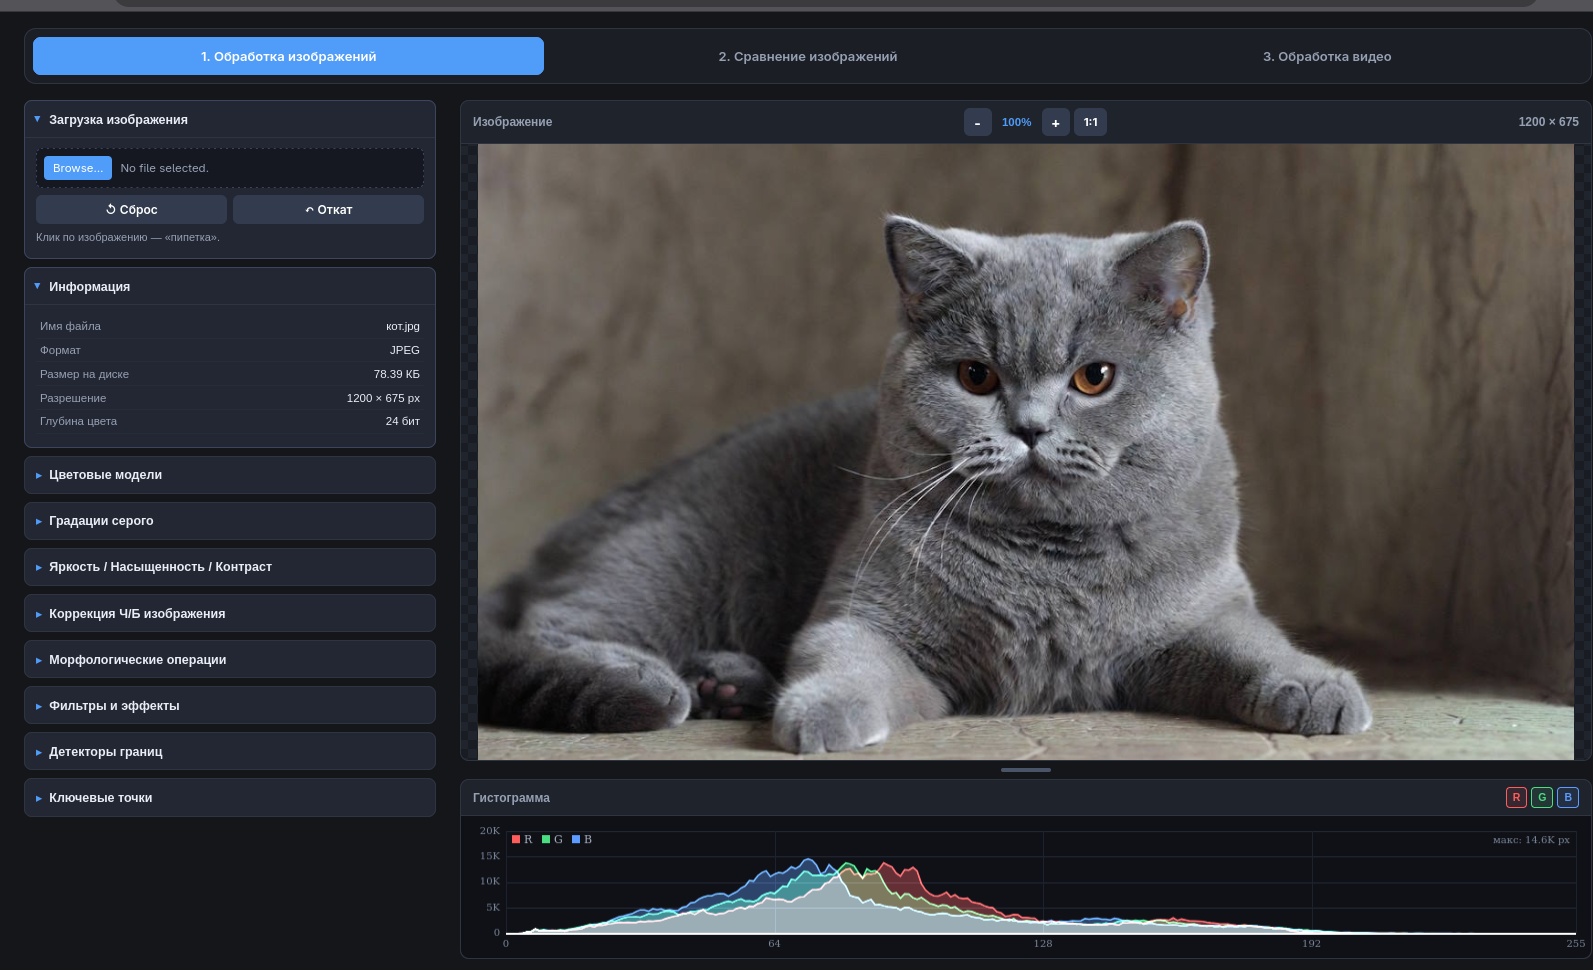
\includegraphics[width=0.8\textwidth]{image.png}
    \caption{Результат работы системы: обработка статического изображения (цветовые преобразования, яркостные преобразования и морфологические операции)}
    \label{fig:result_static}
\end{figure}

\begin{figure}[h!]
    \centering
    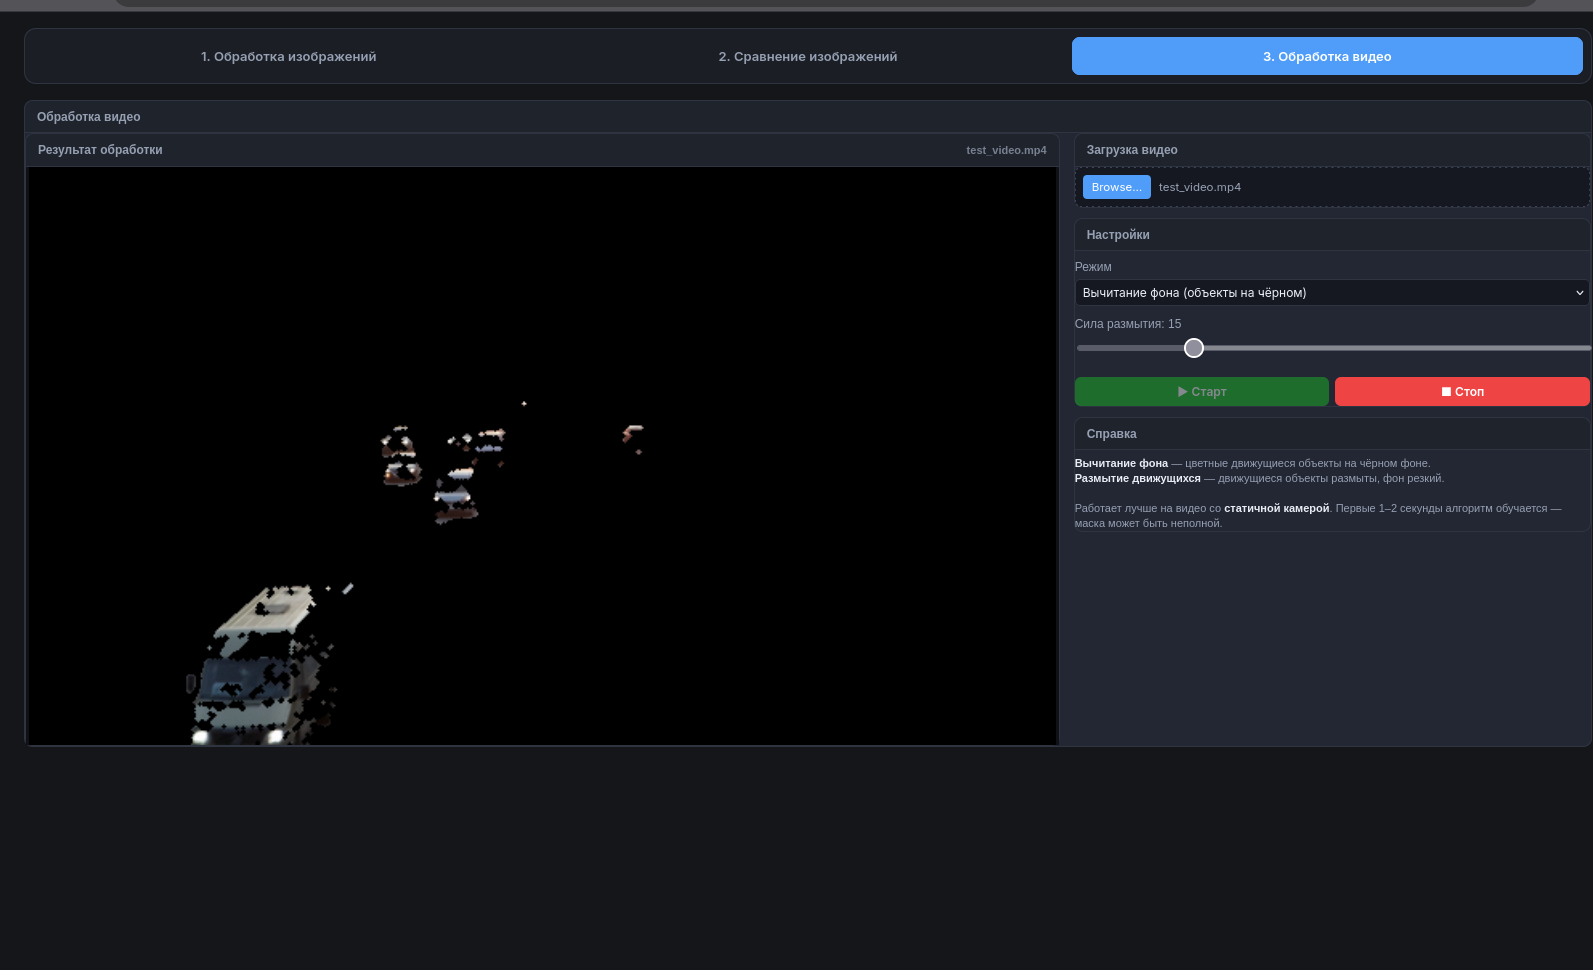
\includegraphics[width=0.8\textwidth]{image1.png}
    \caption{Результат работы системы: анализ видеопотока и поиск похожих изображений}
    \label{fig:result_video}
\end{figure}

Разработанная система позволяет наглядно оценить влияние каждого из рассмотренных методов на исходное изображение и подтверждает корректность формул и алгоритмов, приведённых в теоретической части.

\end{document}